\documentclass[11pt, a4paper]{article}

\usepackage{graphicx}
\usepackage{fullpage}
\usepackage{siunitx}

\begin{document}
\title{FYSS360 Numerical exercise}
\author{Sakari Kapanen}
\date{\today}
\maketitle

A single particle electron model was used to estimate the loss cone of electrons in an ECR ion source. It is also a demonstration of the confinement of electrons (and ions) in a magnetic bottle formed by the generated solenoid and hexapole magnetic fields.

The on-axis solenoid field $B_z(r=0, z)$ and the hexapole field $\mathbf{B}(x, y)$ were plotted (figures~\ref{fig:solenoidb} and~\ref{fig:hexapoleb}).
\begin{figure}
    \centering
    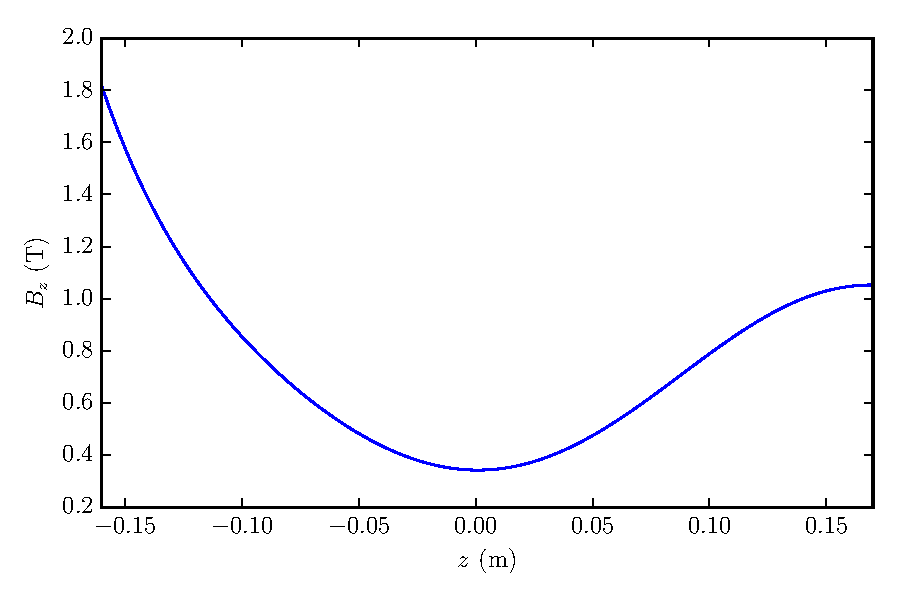
\includegraphics[width=\textwidth]{output/solenoid_B_onaxis.pdf}
    \caption{Solenoid on-axis magnetic field $B_z(r=0, z)$.}
    \label{fig:solenoidb}
\end{figure}
\begin{figure}
    \centering
    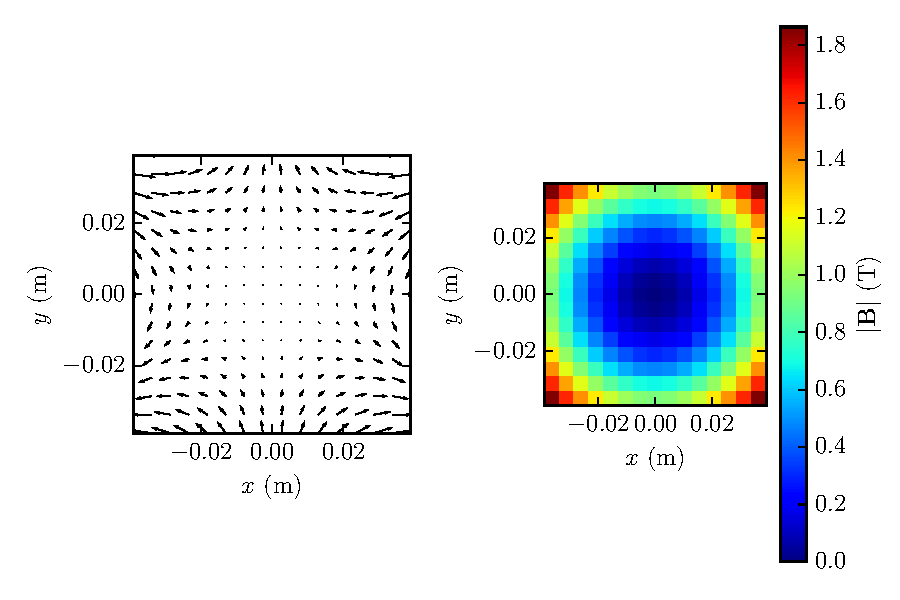
\includegraphics[width=\textwidth]{output/hexapole_B.pdf}
    \caption{The direction and magitude of the hexapole B field.}
    \label{fig:hexapoleb}
\end{figure}
Slices of the total magnetic field were plotted as well at $(x=0, y, z)$ and $(x, y=0, z)$ (figures~\ref{fig:totalb_yz} and~\ref{fig:totalb_xz}).
\begin{figure}
    \centering
    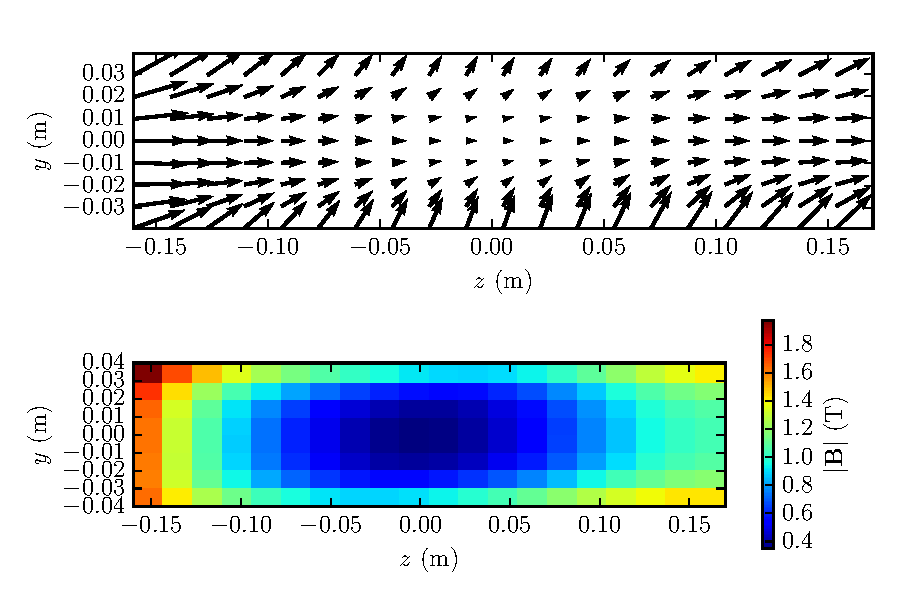
\includegraphics[width=\textwidth]{output/total_B_yz.pdf}
    \caption{A slice of the total magnetic field $\mathbf{B}(x=0, y, z)$. }
    \label{fig:totalb_yz}
\end{figure}
\begin{figure}
    \centering
    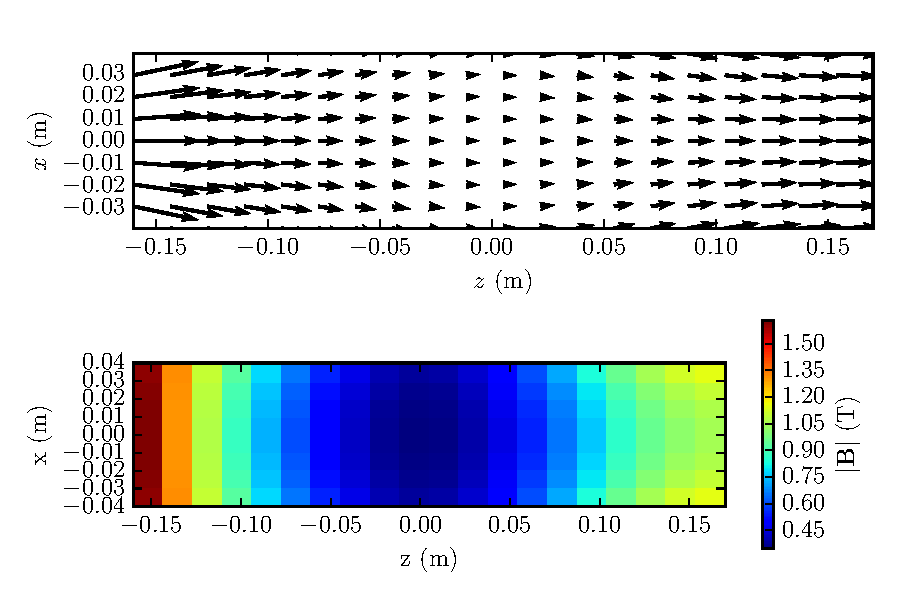
\includegraphics[width=\textwidth]{output/total_B_xz.pdf}
    \caption{A slice of the total magnetic field $\mathbf{B}(x, y = 0, z)$. }
    \label{fig:totalb_xz}
\end{figure}

Electrons with uniform random velocities (with constant energy $10\,\si{\kilo\electronvolt}$) and positions inside the cylindrical plasma chamber ($z_1 = -160\,\si{\milli\meter}$, $z_2 = 170\,\si{\milli\meter}$ and $r = 39\,\si{\milli\meter}$) were generated. Further selection was done with respect to the position: only electrons with position $\mathbf{r}$ such that $|\mathbf{B}(\mathbf{r})| < 0.5\,\si{\tesla}$ were accepted for the simulation --- these correspond to electrons within the ECR zone.

The paths of the electrons were tracked independently, one at a time. The Boris integrator was used to solve the equations of motion in the presence of a static magnetic field. In order to determine the timestep length sufficient to maintain stability, the trajectory of one random particle was tracked for $10^{-8}\,\si{\second}$ and plotted with timestep lengths $10^{-10}$, $10^{-11}$ and $10^{-12}\,\si{\second}$ (figures~\ref{fig:particle10},~\ref{fig:particle11} and~\ref{fig:particle12} respectively).
\begin{figure}
    \centering
    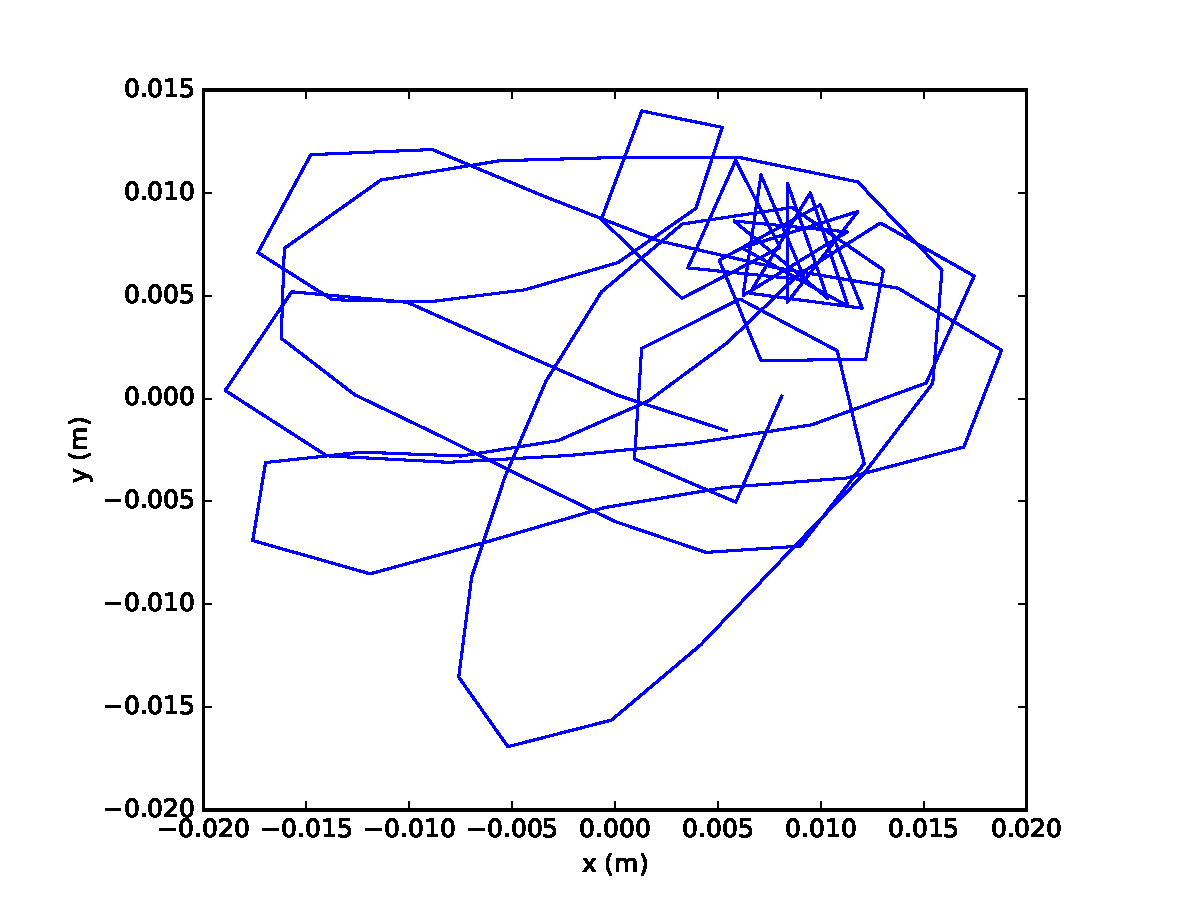
\includegraphics[width=\textwidth]{output/particle_trajectory_10.pdf}
    \caption{The trajectory of a particle with timestep $\Delta t = 10^{-10}\,\si{\second}$.}
    \label{fig:particle10}
\end{figure}
\begin{figure}
    \centering
    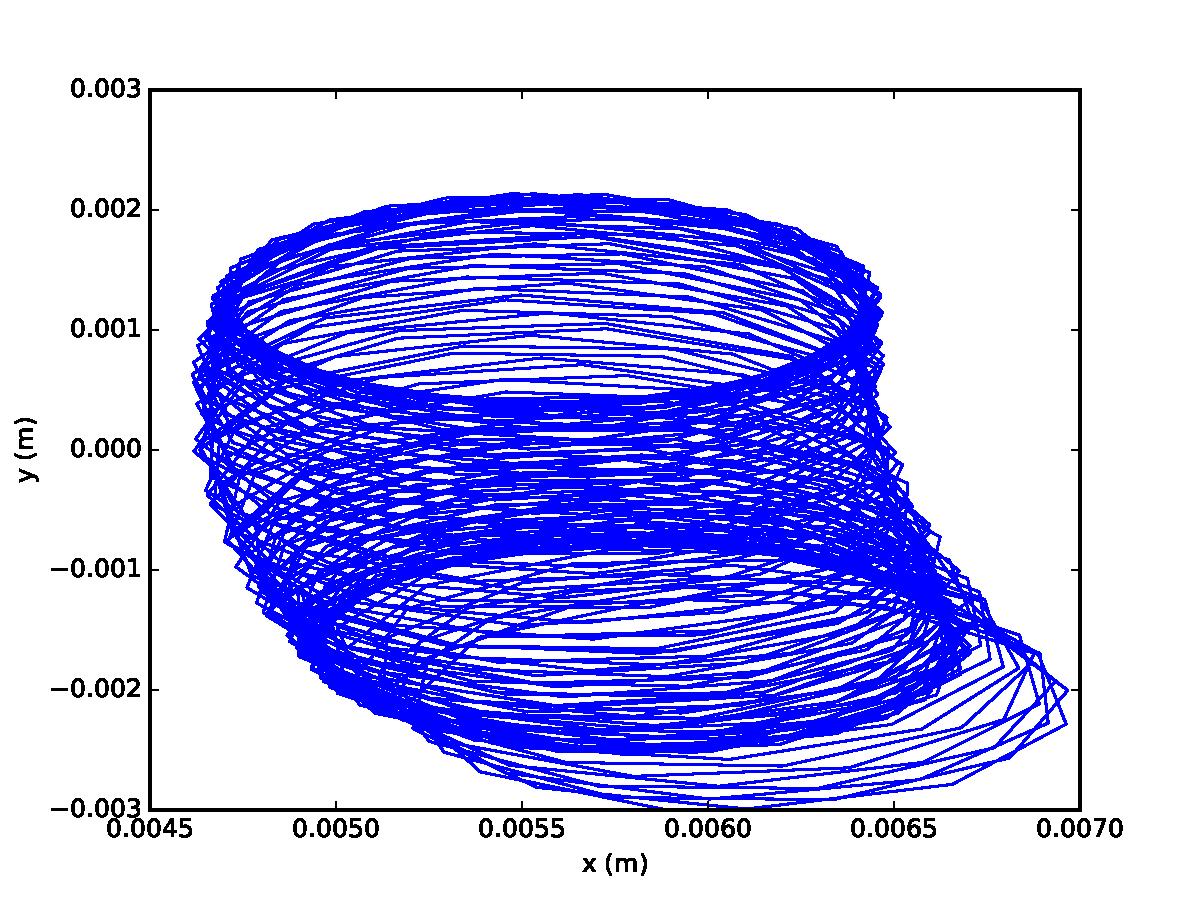
\includegraphics[width=\textwidth]{output/particle_trajectory_11.pdf}
    \caption{The trajectory of a particle with timestep $\Delta t = 10^{-11}\,\si{\second}$.}
    \label{fig:particle11}
\end{figure}
\begin{figure}
    \centering
    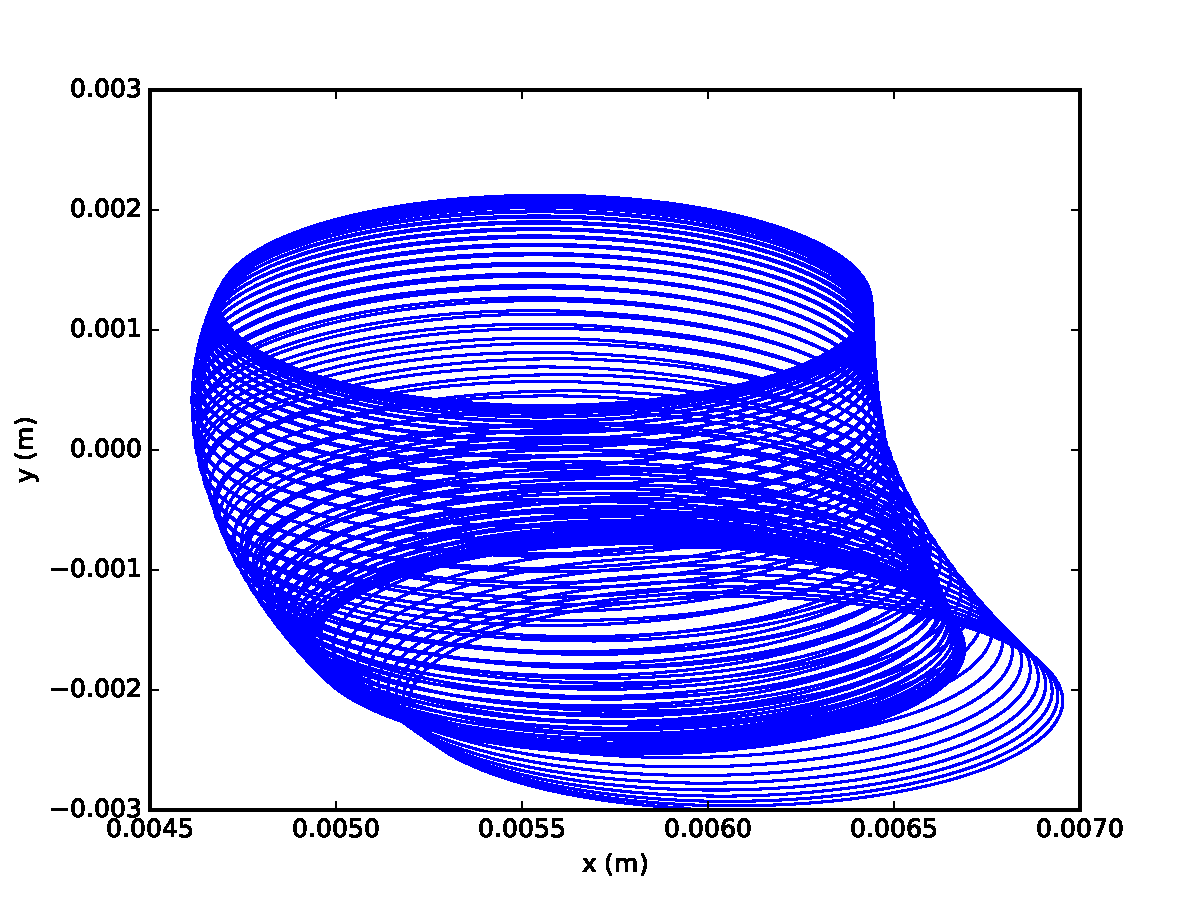
\includegraphics[width=\textwidth]{output/particle_trajectory_12.pdf}
    \caption{The trajectory of a particle with timestep $\Delta t = 10^{-12}\,\si{\second}$.}
    \label{fig:particle12}
\end{figure}
From these figures it is immediately seen that at $\Delta t = 10^{-10}\,\si{\second}$ the solution is unstable. At $\Delta t = 10^{-11}\,\si{\second}$ it seems that for this trajectory stability is achieved. In the end, a timestep length $\Delta t = 5\times 10^{12}\,\si{\second}$ was chosen in order to have a safety margin.

In order to have sufficient statistics, the number of test particles was chosen to be $N=10^5$. Particles were tracked until they hit any of the cylinder ends and walls or the confinement time of $10^{-6}\,\si{\second}$ was elapsed. The locations where the electrons hit the geometry were recorded. Histograms for the end circles at $z_1 = -160\,\si{\milli\meter}$ and $z_2 = 170\,\si{\milli\meter}$ and the radial wall are shown in figures~\ref{fig:z_1_coll},~\ref{fig:z_2_coll} and~\ref{fig:wall} respectively.
\begin{figure}
    \centering
    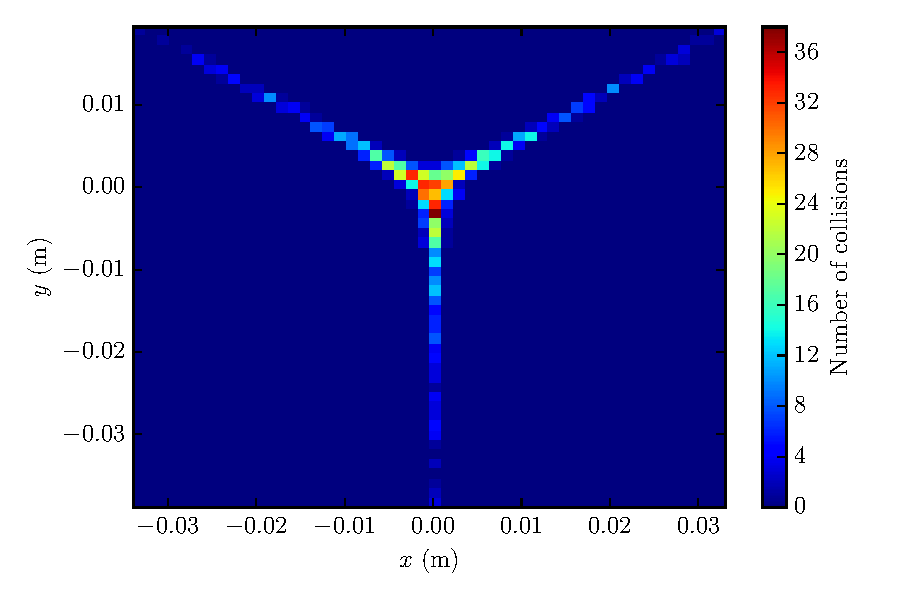
\includegraphics[width=\textwidth]{output/z1_collision_points.pdf}
    \caption{Histogram of electron collision locations at the end circle $z_1=-160\,\si{\milli\meter}$.}
    \label{fig:z_1_coll}
\end{figure}
\begin{figure}
    \centering
    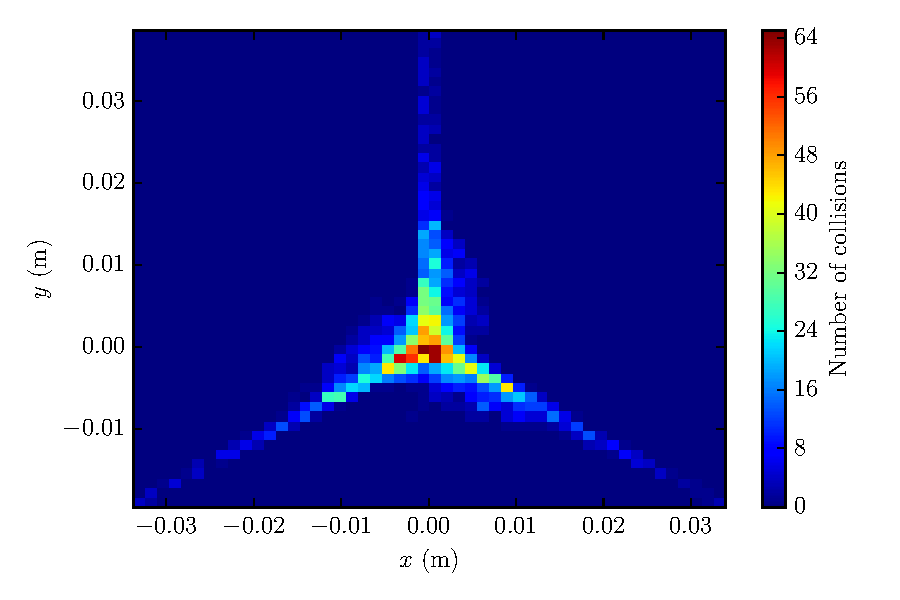
\includegraphics[width=\textwidth]{output/z2_collision_points.pdf}
    \caption{Histogram of electron collision locations at the end circle $z_2=170\,\si{\milli\meter}$.}
    \label{fig:z_2_coll}
\end{figure}
\begin{figure}
    \centering
    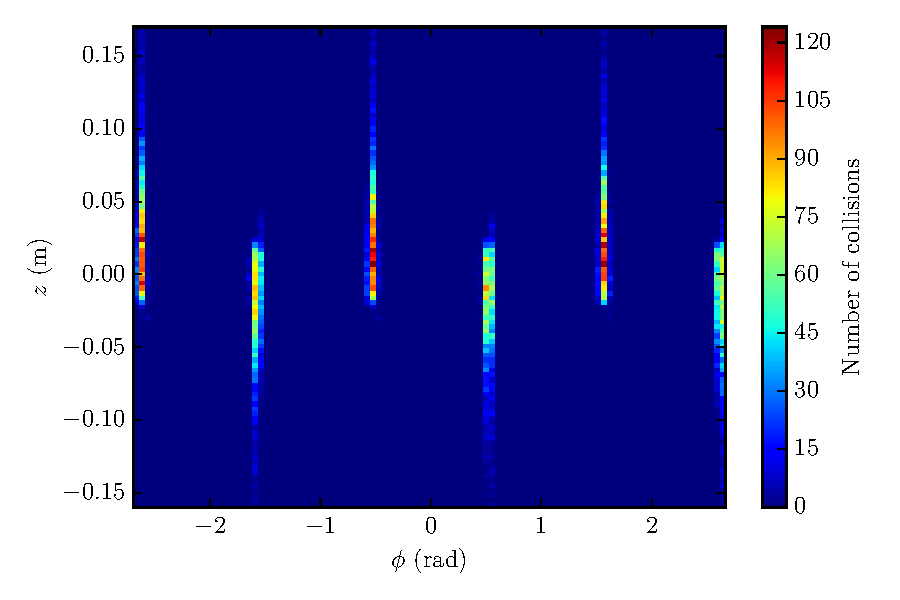
\includegraphics[width=\textwidth]{output/cylinder_collision_points.pdf}
    \caption{Histogram of electron collision locations at the wall of the cylinder.}
    \label{fig:wall}
\end{figure}

In the simulation, the radial and transverse components $(v_\parallel, v_\perp)$ of the particle starting velocities w.r.t. $\mathbf{B}$ field were logged. These are plotted in figure~\ref{fig:vel} separately for lost and non-lost particles. From there one can determine the loss cone angle.

\end{document}

